\section{Descrição Geral do Sistema}
O sistema proposto consiste em uma prótese robótica de mão e braço controlada por sinais de eletromiografia de superfície, com comunicação sem fio entre dois módulos ESP32. A Figura \ref{fig:Fluxograma} ilustra a arquitetura geral do sistema, composta pelos seguintes subsistemas:
\begin{itemize}
    \item Módulo de aquisição: eletrodos sEMG posicionados sobre os músculos do antebraço do usuário, conectados a um circuito de condicionamento de sinal (amplificação e filtragem), cuja saída é digitalizada pelo ESP32 transmissor;
    \item Módulo de processamento e comunicação: o ESP32 transmissor realiza a segmentação das janelas de sinal, a extração de características e a classificação do gesto por meio do modelo de aprendizado de máquina embarcado, transmitindo o rótulo do gesto reconhecido via ESP-NOW ao ESP32 receptor;
    \item Módulo de controle da prótese: o ESP32 receptor recebe o comando de gesto e aciona os servomotores por sinais PWM, reproduzindo o movimento correspondente.   

\end{itemize}
 \begin{figure}[htbp]
    \centering
    \caption{Fluxograma do funcionamento geral}
    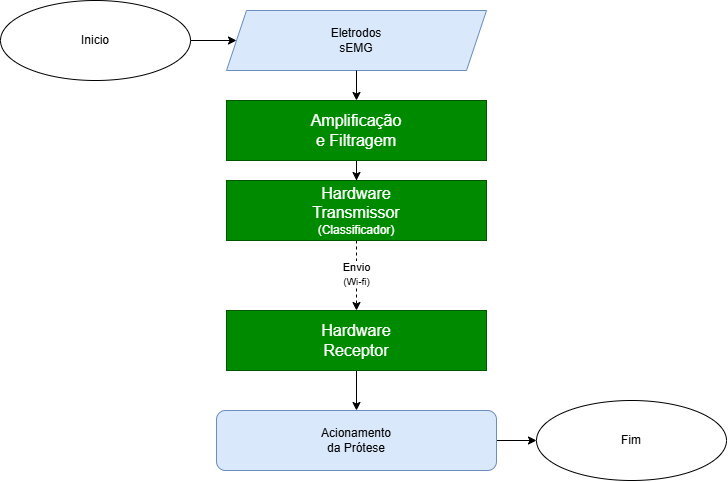
\includegraphics[width=1\textwidth]{3_proposta_desenvolvimento/assets/FluxogramaGeralHorizontal.png}
    \fonte{Elaborado pelo autor (2026)}
    \label{fig:Fluxograma}
\end{figure}